\documentclass[11pt, twoside, pdftex]{article}

% This includes all the settings that we should use for the document
\newcommand{\PDFTitle}{Using the Questa Intel FPGA Simulator with VHDL Testbenches}
\newcommand{\commonPath}{../../../Common}
\newcommand{\datePublished}{Mar 2022}

\newcommand{\versnum}{21.1} %version number quartus/AMP
\newcommand{\quartusname}{Quartus\textsuperscript{\textregistered} Prime}	
\newcommand{\textBar}{For \quartusname{} \versnum{}}
\newcommand{\thisyear}{2022 } %for copyright
\newcommand{\company}{FPGAcademy.org}
\newcommand{\longteamname}{FPGAcademy.org}
\newcommand{\teamname}{FPGAcademy}
\newcommand{\website}{FPGAcademy.org}

\newcommand{\productAcronym}{AMP}
\newcommand{\productNameShort}{Monitor Program}

\newcommand{\productNameMedTM}{Monitor Program}
\newcommand{\productNameMed}{Monitor Program}

%\newcommand{\headerLogoFilePath}[1]{#1/FPGAcademy.png}



\setlength\topmargin{-0.25in}
\setlength\headheight{0in}
\setlength\headsep{0.35in}
\setlength\textheight{8.5in}
\setlength\textwidth{7in}
\setlength\oddsidemargin{-0.25in}
\setlength\evensidemargin{-0.25in}
\setlength\parindent{0.25in}
\setlength\parskip{0in} 

\pdfpagewidth 8.5in
\pdfpageheight 11in

% listings is a package that supports encapsulating source code in LaTeX conveniently

\usepackage{listings}
% add support for graphics
\usepackage{graphicx}
\usepackage[usenames, dvipsnames]{color}

\def\expandparam\lstinputlisting[#1]#2{\edef\tmp{\noexpand\lstinputlisting[#1]{#2}}\tmp}

\widowpenalty 10000
\clubpenalty 10000

%%%%%%%%%%%%%%%%%%%% Source Code Formatting %%%%%%%%%%%%%%%%%%%%
\definecolor{globalCommentColour}{rgb}{0.588,0.588,0.588}

%%%%%%%%%%%%%%%%%%%%%%%%%%%%%%%%%%%%%%%%%%%%%%%%%%%%
% Defining a NiosII ASM highlighter for lstlisting
\lstdefinelanguage[NiosII]{Assembler} {
 	morekeywords={add, addi, and, andhi, andi, beq, bge, bgeu, bgt, bgtu, ble,  bleu, blt, bltu, bne, br, break,% 
 	bret, call, callr, cmpeq, cmpeqi, cmpge, cmpgei, cmpgeu, cmpgeui, cmpgt, cmpgti, cmpgtu, cmpgtui, cmple,%
 	cmplei, cmpleu, cmpleui, cmplt, cmplti, cmpltu, cmpltui, cmpne, cmpnei, custom, div, divu, eret, flushd,%
 	flushda, flushi, flushp, initd, initda, initi, jmp, jmpi, ldb, ldbio, ldbu, ldbuio, ldh, ldhio, ldhu, ldhuio,%
 	ldw, ldwio, mov, movhi, movi, movia, movui, mul, muli, mulxss, mulxsu, mulxuu, nextpc, nop, nor, or, orhi, ori,%
 	rdctl, rdprs, ret, rol, roli, ror, sll, slli, sra, srai, srl, srli, stb, stbio, sth, sthio, stw, stwio,%
 	sub, subi, sync, trap, wrctl, wrtcl, wrprs, xor, xori, xorhi, xori},% 	
 	morekeywords=[2]{.abort, .ABORT, .align, .app-file, .ascii, .asciz, .balign, .byte, .comm, .data, .def,%
 	.desc, .dim, .double, .eject, .else, .end, .endef, .endif, .equ, .equiv, .err, .extern, .file, .fill, .float,%
 	.global, .globl, .hword, .ident, .if, .include, .int, .irp, .irpc, .lcomm, .lflags, .line, .linkonce, .ln,%
 	.list, .long, .macro, .mri, .nolist, .octa, .org, .p2align, .psize, .quad, .rept, .sbttl, .scl, .section,%
 	.set, .short, .single, .size, .sleb128, .skip, .space, .stadb, .stabn, .stabs, .string, .symver, .tag,%
 	.text, .title, .type, .val, .uleb128, .word},% 	
 	morekeywords=[3]{et, bt, gp, sp, fp, ea, sstatus, ra, pc, status, estatus, bstatus, ienable, ipending, cpuid,%
 	exception, pteaddr, tlbacc, tlbmisc, eccinj, badaddr, config, mpubase, mpuacc},% 	
 	sensitive=t,%
 	alsoletter=.,%
	morestring=[b]",%
 	morecomment=[s]{/*}{*/},%
 	morecomment=[l]\#,%
   }[keywords,comments,strings]
   
   %% NOTE: morekeywords=[2] are GNU directives.
   
   \definecolor{niosInstructionColour}{rgb}{0.000,0.608,0.000}
   \definecolor{niosDirectiveColour}{rgb}{0.000,0.000,0.902}
   \definecolor{niosSpecialRegColour}{rgb}{0.000,0.000,0.000}
   \definecolor{niosStringColour}{rgb}{0.808,0.482,0.000}
   
   %% NOTE: To make bold use: =\bfseries\color{<colour>}
   \lstdefinestyle{defaultNiosStyle} {
   language=[NiosII]{Assembler},
   stringstyle=\color{niosStringColour},
   keywordstyle=\color{niosInstructionColour},
   keywordstyle=[2]\color{niosDirectiveColour},
   keywordstyle=[3]\itshape\color{niosSpecialRegColour}
   }
%%%%%%%%%%%%%%%%%%%%%%%%%%%%%%%%%%%%%%%%%%%%%%%%%%%%

%%%%%%%%%%%%%%%%%%%%%%%%%%%%%%%%%%%%%%%%%%%%%%%%%%%%
% Defining a ArmA9 ASM highlighter for lstlisting
\lstdefinelanguage[ArmA9]{Assembler} {
 	morekeywords={ADC, ADD, ADDS, AND, ANDS, B, BAL, BEQ, BGE, BGT, BL, BLT, BIC, BKPT, BLX, BNE, BX, CDP, CLZ, CMN, CMP, EOR,%
 	EORS, LDC, LDM, LDR, LDRB, LDRBT, LDRH, LDRSB, LDRSH, LDRT, LSL, MCR, MLA, MOV, MOVW, MOVT, MRC, MRS, MSR, MUL, MVN, ORR, PLD,%
 	ROR, RSB, RSC, SBC, SMLAL, SMULL, STC, STM, STR, STRB, STRBT, STRH, STRT, SUB, SUBS, SWI, SWP, SWPB, TEQ, UMLAL,
 	PUSH, POP, MOVS, RORS, LSR},%
 	morekeywords=[2]{.abort, .ABORT, .align, .app-file, .ascii, .asciz, .balign, .byte, .comm, .data, .def,%
 	.desc, .dim, .double, .eject, .else, .end, .endef, .endif, .equ, .equiv, .err, .extern, .file, .fill, .float,%
 	.global, .globl, .hword, .ident, .if, .include, .int, .irp, .irpc, .lcomm, .lflags, .line, .linkonce, .ln,%
 	.list, .long, .macro, .mri, .nolist, .octa, .org, .p2align, .psize, .quad, .rept, .sbttl, .scl, .section,%
 	.set, .short, .single, .size, .sleb128, .skip, .space, .stadb, .stabn, .stabs, .string, .symver, .tag,%
 	.text, .title, .type, .val, .vectors, .uleb128, .word},%
 	morekeywords=[3]{SP, PC, MIDR, CTR, TCMTR, TLBTR, MPIDR, ID_PFR0, ID_PFR1, ID_DFR0, ID_MMFR0, ID_MMFR1, ID_MMFR2,%
 	ID_MMFR3, ID_ISAR0, ID_ISAR1, ID_ISAR2, ID_ISAR3, ID_ISAR4, CCSIDR, CLIDR, AIDR, CSSELR, TTBR0, TTRB1, TTBR2, DACR,%
 	DFSR, IFSR, ADFSR, AIFSR, DFAAR, IFAR, ICIALLUIS, BPIALLIS, PAR, ICIALLU, ICIMVAU, BPIALL, DCIMVAC, DCISW, V2PCWPR,%
 	DCCVAC, DCCSW, DDIMVAC, DCISW, TLBALLIS, TLBIMVAIS, TLBIASIDIS, TLBIMVAAIS, TLBIALL, TLBIMVA, TLBIASID, TLBIMVAA,%
 	PMCR, PMCNTENSET, PMCNTENCLR, PMOVSR, PMSWINC, PMSELR, PMXEVTYPER, PMXEVCNTR, PMUSERENR, PMINTENSET, PMINTENCLR,%
 	PRRR, NRRR, PLEIDR, PLEASR, PLEFSR, PLEUAR, PLEPCR, VBAR, MVBAR, ISR, FCSEIDR, CONTEXTIDR, TPIDRURW, TPIDRURO, TPIDRPRW},%
 	sensitive=f,%
 	alsoletter=.,%
	morestring=[b]",%
 	morecomment=[s]{/*}{*/},%
 	morecomment=[l]{//},%
   }[keywords,comments,strings]
   
   %% NOTE: morekeywords=[2] are GNU directives.
   
   \definecolor{armInstructionColour}{rgb}{0.000,0.608,0.000}
   \definecolor{armDirectiveColour}{rgb}{0.000,0.000,0.902}
   \definecolor{armSpecialRegColour}{rgb}{0.000,0.000,0.000}
   \definecolor{armStringColour}{rgb}{0.808,0.482,0.000}
   
   \lstdefinestyle{defaultArmStyle} {
   language=[ArmA9]{Assembler},
   stringstyle=\color{armStringColour},
   keywordstyle=\color{armInstructionColour},
   keywordstyle=[2]\color{armDirectiveColour},
   keywordstyle=[3]\itshape\color{armSpecialRegColour}
   }
%%%%%%%%%%%%%%%%%%%%%%%%%%%%%%%%%%%%%%%%%%%%%%%%%%%%

%%%%%%%%%%%%%%%%%%%%%%%%%%%%%%%%%%%%%%%%%%%%%%%%%%%%
% Defining style for the verilog.

\definecolor{verilogCommentColour}{rgb}{0.000,0.502,0.000}

\lstdefinestyle{defaultVerilogStyle} {
language={Verilog},
keywordstyle=\color{blue},
commentstyle=\color{verilogCommentColour}
}
%%%%%%%%%%%%%%%%%%%%%%%%%%%%%%%%%%%%%%%%%%%%%%%%%%%%

%%%%%%%%%%%%%%%%%%%%%%%%%%%%%%%%%%%%%%%%%%%%%%%%%%%%
% Defining style for the vhdl.
\lstdefinestyle{defaultVHDLStyle} {
language={VHDL},
keywordstyle=\color{blue},
commentstyle=\color{verilogCommentColour}
}
%%%%%%%%%%%%%%%%%%%%%%%%%%%%%%%%%%%%%%%%%%%%%%%%%%%%

%%%%%%%%%%%%%%%%%%%%%%%%%%%%%%%%%%%%%%%%%%%%%%%%%%%%
% Java
\definecolor{javaStringColour}{rgb}{0.808,0.482,0}
%%%%%%%%%%%%%%%%%%%%%%%%%%%%%%%%%%%%%%%%%%%%%%%%%%%%

%%%%%%%%%%%%%%%%%%%%%%%%%%%%%%%%%%%%%%%%%%%%%%%%%%%%
% Defining language styles
% C
\definecolor{CStringColour}{rgb}{0.808,0.482,0}
%%%%%%%%%%%%%%%%%%%%%%%%%%%%%%%%%%%%%%%%%%%%%%%%%%%%

%%%%%%%%%%%%%%%%%%%%%%%%%%%%%%%%%%%%%%%%%%%%%%%%%%%%
% Defining extended LaTeX language.
\lstdefinelanguage[LocalLaTeX]{TeX}[LaTeX]{TeX}%
 	{moretexcs={bf, it, sf, lstset},%
   	}%

\lstdefinestyle{defaultLocalLatexStyle} {
language=[LocalLatex]{TeX},
keywordstyle=\color{blue}\bfseries,
keywordstyle=[2]\color{blue},
keywordstyle=[3]\color{blue}\bfseries
}
%%%%%%%%%%%%%%%%%%%%%%%%%%%%%%%%%%%%%%%%%%%%%%%%%%%%

\lstset{
%language = C,
%language = Verilog,
%basicstyle=\color{black}\rmfamily\ttfamily,
basicstyle=\small\color{black}\ttfamily,
commentstyle=\small\color{globalCommentColour}\itshape\ttfamily,
keywordstyle=\small\color{blue}\bfseries\ttfamily,
showstringspaces=false,
frame=none, %lines % boxed listings
breaklines=true,
breakatwhitespace=true,
tabsize=4
}
%%%%%%%%%%%%%%%%%%%%%%%%%%%%%%%%%%%%%%%%%%%%%%%%%%%%%%%%%%%%%%%%


%\usepackage[centering]{geometry}.
%%%%%%%%%%%%%%%%%%%%%%%%%%%%%%%%%%%%%%%%%%%%%%%%%%%
% Document Settings
\usepackage[labelsep=period]{caption}
% we can choose a better font later
%\usepackage{palatino}
\usepackage{fourier}
%\fontencoding{T1}
% include common used symbols
\usepackage{textcomp}
% add support for graphics
\usepackage{graphicx}
\usepackage[usenames, dvipsnames]{color}
% enable to draw thick or thin table hlines
\setlength{\doublerulesep}{\arrayrulewidth}
\usepackage{longtable}
\setlongtables
%\usepackage{array}
% It may be better to use PDFLaTeX as it can generate bookmarks for the
% document

% Add some useful packages
\usepackage{ae,aecompl}
\usepackage{epsfig,float,times}

% reset the font for section
\usepackage{sectsty}
%\allsectionsfont{\fontfamily{ptm}\selectfont}
\allsectionsfont{\usefont{OT1}{phv}{bc}{n}\selectfont}

% use compact space for sections
\usepackage[compact]{titlesec}
\titlespacing{\section}{0pt}{0.2in}{*0}
\titlespacing{\subsection}{0pt}{0.1in}{*0}
\titlespacing{\subsubsection}{0pt}{0.05in}{*0}

% fancyhdr header and footer customization
\usepackage{layout}
\usepackage{fancyhdr}
\pagestyle{fancy}
\fancyhead{}
\fancyhead[R]{\textit{\tiny{\textBar}}}
\fancyfoot{}
\fancyfoot[LO,
RE]{\textrm{\href{https://www.fpgacademy.org}{\small \longteamname}} \\ {\small \datePublished }}
\fancyfoot[RO, LE]{\small \thepage}
% two-side settings
%\fancyhead{} % clear all header fields
%\fancyfoot{} % clear all footer fields
%\fancyfoot[LE,RO]{\thepage}
\renewcommand{\headrulewidth}{2pt}
\renewcommand{\headrule}{{\color{blue} \hrule width\headwidth height\headrulewidth \vskip-\headrulewidth}}
\renewcommand{\footrulewidth}{0pt}

% Format the footer on page 1
\fancypagestyle{plain}{
\fancyhead{}
\fancyfoot{}
\fancyfoot[LO,
RE]{\textrm{\href{https://www.fpgacademy.org}{\small \longteamname}} \\ {\small \datePublished }}
\fancyfoot[RO, LE]{\small \thepage}
\renewcommand{\headrulewidth}{0pt}
}
% adjust some setting to try to make the figure stay in the same page with text
% Reference: 	http://www.cs.uu.nl/~piet/floats/node1.html
%   			http://mintaka.sdsu.edu/GF/bibliog/latex/floats.html
%   General parameters, for ALL pages:
\renewcommand{\topfraction}{0.9}	% max fraction of floats at top
\renewcommand{\bottomfraction}{0.8}	% max fraction of floats at bottom
%   Parameters for TEXT pages (not float pages):
\setcounter{topnumber}{3}
\setcounter{bottomnumber}{3}
\setcounter{totalnumber}{5}     % 2 may work better
\setcounter{dbltopnumber}{2}    % for 2-column pages
\renewcommand{\dbltopfraction}{0.9}	% fit big float above 2-col. text
\renewcommand{\textfraction}{0.07}	% allow minimal text w. figs
%   Parameters for FLOAT pages (not text pages):
\renewcommand{\floatpagefraction}{0.7}	% require fuller float pages
% N.B.: floatpagefraction MUST be less than topfraction !!
\renewcommand{\dblfloatpagefraction}{0.7}	% require fuller float pages
%%%%%%%%%%%%%%%%%%%%%%%%%%%%%%%%%%%%%%%%%%%%%%%%%%%
% remember to use [htp] or [htpb] for placement
%%%%%%%%%%%%%%%%%%%%%%%%%%%%%%%%%%%%%%%%%%%%%%%%%%%

% set no indent for paragraph
\setlength{\parindent}{0em}
\addtolength{\parskip}{11pt}
\newcommand{\compact}{[topsep=0pt]}
% use this package to reduce space
\usepackage{enumitem}
\usepackage{multirow}
\usepackage{rotating}
\usepackage{pifont}
\usepackage{dingbat}
\newcommand{\itemsecond}{$\circ$}
%
%%%%%%%%%%%%%%%%%%
\date{}
\author{}
%%%%%%%%%%%%%%%%%%
\newcommand{\de}{DE-series}
\newcommand{\up}{FPGAcademy}
\newcommand{\fabric}{Avalon Switch Fabric}
\newcommand{\TODO}[1]{\textcolor{red}{\textbf{TODO}: #1}}
\def\registered{{\ooalign{\hfil\raise .00ex\hbox{\scriptsize R}\hfil\crcr\mathhexbox20D}}}

% enable url and reference(bookmarks) in pdf
\usepackage{url}
\usepackage[pdftex, colorlinks]{hyperref}
\hypersetup{%
pdftitle={\PDFTitle},
linkcolor=blue,
hyperindex=true,
pdfauthor={\longteamname},
pdfkeywords={FPGAcademy, Academic Program, Example System},
bookmarksnumbered,
bookmarksopen=false,
filecolor=blue,
pdfstartview={FitH},
urlcolor=blue,
plainpages=false,
pdfpagelabels=true,
linkbordercolor={1 1 1} %no color for link border
}%
%%%%%%%%%%%%%%%%%%%%%%%%%%%%%%%%%%%%%%%%%%%%%%%%%%%
\setlength{\fboxsep}{0.7pt}
\setlength{\fboxrule}{0.5pt}

\newcommand{\red}[1]{{\color{red}\sf{#1}}}
\newcommand{\blue}[1]{{\color{blue}\sf{#1}}}



\usepackage{placeins}

%%%%%%%%%%%%%%%%%%%%%%%%%
% Add title
\newcommand{\doctitle}{Using the Questa Intel FPGA \\ Simulator with VHDL Testbenches}
\newcommand{\dochead}{Using the Questa Intel FPGA Simulator with VHDL Testbenches}
% Usually no need to change these two lines
\title{\fontfamily{phv}\selectfont{\doctitle} }
\chead{ \small{\textsc{\bfseries \dochead} } }
% Customizations
%%%%%%%%%%%%%%%%%%%%%%%%%
% Allows multiple figures per page

\renewcommand\floatpagefraction{.9}
\renewcommand\topfraction{.9}
\renewcommand\bottomfraction{.9}
\renewcommand\textfraction{.1}   
\setcounter{totalnumber}{50}
\setcounter{topnumber}{50}
\setcounter{bottomnumber}{50}
\raggedbottom

%%%%%%%%%%%%%%%%%%
%%% DOCUMENT START
%\begin{document}
\begin{document}
\begin{table}
    \centering
    \begin{tabular}{p{5cm}p{4cm}}
	\hspace{-3cm}
        &
        \raisebox{1\height}{\parbox[h]{0.5\textwidth}{\Large\fontfamily{phv}\selectfont{\textsf{\doctitle}}}}
    \end{tabular}
    \label{tab:logo}
\end{table}

\colorbox[rgb]{0,0.384,0.816}{\parbox[h]{\textwidth}{\color{white}\textsf{\textit{\textBar}}}}

\thispagestyle{plain}
\newcommand{\red}[1]{{\color{red}\sf{#1}}}
\lstset{language=VHDL}

\section{Introduction}

This tutorial introduces the simulation of VHDL code using the
{\it Questa Intel FPGA} simulator. We assume 
that you are using {\it Questa Intel Starter FPGA Edition-64 2021.2}. This software can 
be downloaded and installed from the {\it Download Center for Intel FPGAs}. In this
download center, you can select release {\it \versnum} of the {\it Quartus Prime Lite Edition}, 
and then on the \texttt{Individual Files} tab choose to download and install the 
{\it Questa Intel FPGA Starter Edition} software. We assume that you are using a computer
that is running the Windows operating system. If you are using the Linux operating system 
then minor differences to the instructions would apply, such as using a / filesystem delimiter 
rather than the $\backslash$ delimiter that is used with Windows. 
 
{\bf Contents:}
\begin{itemize}
\item Getting Started with Questa
\item Simulating a Sequential Circuit
\item Simulating a Circuit that Includes a Memory Module
\item Setting up a Questa Simulation
\item Using the Questa Graphical User Interface
\end{itemize}

{\bf Requirements:}
\begin{itemize}
\item Questa Intel FPGA Starter Edition software
\item A computer running either Microsoft* Windows* (version 10 is recommended) or Linux 
(Ubuntu, or a similar Linux distribution). The computer would typically be either a
desktop computer or laptop, and is used to run the Questa software.
\end{itemize}

{\bf Optional:}
\begin{itemize}
\item Intel Quartus\textsuperscript{\textregistered} Prime software
\item A DE-series development and education board, such as the DE1-SoC board. These boards are 
described on Intel's FPGA University Program website, and are available from the manufacturer 
Terasic Technologies.
\end{itemize}

\clearpage
\newpage
\section{Getting Started}

The Questa Simulator is a sophisticated and powerful tool that supports a variety of 
usage models. In this tutorial we focus on only one design flow: using the Questa
software as a {\it stand-alone} program to perform {\it functional} simulations, with 
simulation inputs specified in a {\it testbench}, and with simulator commands provided 
via {\it script} files. Other possible design flows for using Questa include {\it invoking}
it from within the Intel Quartus Prime software, performing {\it timing} simulations, and
specifying simulation inputs by {\it drawing} waveforms in a graphical editor instead of
using a testbench. These flows are described in other
documentation that is available on the Internet.  

\noindent
To introduce the {\it Questa} software, we will first open an existing simulation example.
The example is a multibit adder named {\it Addern}, and is included as 
part of the {\it design files} provided
along with this tutorial. Copy the {\it Addern} files to a folder on your computer, such
as {\it C:$\backslash$Questa\_Tutorial$\backslash$Addern}. In the {\it Addern} folder
there is a VHDL source-code file called {\it Addern.vhd} and a subfolder named {\it Questa}.
The {\it Addern.vhd} file, shown in Figure~\ref{fig:addern}, is the VHDL code that will 
be simulated in this part of the tutorial. We will specify signal 
values for the adder's inputs, {\it Cin}, {\it X}, and {\it Y}, and then the {\it
Questa} simulator will generate corresponding values for the outputs, {\it S} and {\it Cout}.

\lstset{language=VHDL,numbers=none,escapechar=|}
\begin{figure}[h]
\begin{center}
\begin{minipage}[t]{12.5 cm}
\begin{lstlisting}[name=addern]
library IEEE;
use IEEE.std_logic_1164.all;
use IEEE.std_logic_signed.all;

ENTITY Addern IS 
   GENERIC (n : INTEGER := 16);
   PORT ( X, Y : IN STD_LOGIC_VECTOR(n-1 DOWNTO 0);
          Cin  : IN STD_LOGIC;
          S    : OUT STD_LOGIC_VECTOR(n-1 DOWNTO 0);
          Cout : OUT STD_LOGIC);
END Addern;

ARCHITECTURE Behaviour OF Addern IS 
   SIGNAL Sum : STD_LOGIC_VECTOR(n DOWNTO 0);
BEGIN 
   Sum <= ('0' & X) + ('0' & Y) + Cin;
   S <= Sum(n-1 DOWNTO 0);
   Cout <= Sum(16);
END Behaviour;
\end{lstlisting}
\end{minipage}
\caption{VHDL code for the multibit adder.}
\label{fig:addern}
\end{center}
\end{figure}

\noindent
We will use three files, included in the {\it Questa} subfolder, to control the 
{\it Questa} simulator. The files are named {\it testbench.vht}, {\it testbench.tcl}, and 
{\it wave.do}.

\noindent
The {\it testbench.vht} file is a style of VHDL code known as a {\it testbench}. 
The purpose of a testbench is to {\it instantiate} a VHDL entity that is to be simulated,
and to specify values for its inputs at various simulation times. In this case the module
to be simulated is our multibit adder, which we refer to as the {\it design under test} (DUT).
Line~\ref{line:tb1_entity} is the start of the testbench entity, which has no inputs or
outputs. Line~\ref{line:tb1_component} declares the {\it Addern} component, which will be 
instantiated later in the testbench code. In Lines~\ref{line:tb1_tb1} to \ref{line:tb1_tb2} we 
declare signals to drive the adder inputs {\it Cin}, {\it X}, and~{\it Y}.
Lines~\ref{line:tb1_tb3} and \ref{line:tb1_tb4} declare signals to connect to the 
adder outputs {\it S} and {\it Cout}.

\noindent
Lines~\ref{line:tb1_v1} to \ref{line:tb1_v8} provide a process labeled \texttt{vectors} that is used
to specify the values of the adder inputs. First, in Line~\ref{line:tb1_v2} the adder inputs 
{\it X}, {\it Y}, and {\it Cin} are set to 0. The next line of code waits until 20 ns of 
simulation time has passed, and then line~\ref{line:tb1_v3} changes the input {\it Y} to the 
10.  Following another 20 ns of waiting time, meaning at 40~ns in simulation time, 
line~\ref{line:tb1_v4} changes the input {\it X} to 10. The rest of the
process specifies various values for the adder inputs at 20 ns time increments.
Finally, in Line~\ref{line:tb1_addern} the {\it testbench} entity instantiates the {\it Addern} entity. Its inputs are driven by the testbench signal values specified in the \texttt{vectors} process. 

\lstset{language=VHDL,numbers=left,escapechar=|}
\begin{figure}[h!]
\begin{center}
\begin{minipage}[t]{15 cm}
\begin{lstlisting}[name=testbench]
LIBRARY ieee;                                               
USE ieee.std_logic_1164.all;                                
USE ieee.std_logic_signed.all;

|\label{line:tb1_entity}|ENTITY testbench IS
END testbench;

ARCHITECTURE Behavior OF testbench IS
|\label{line:tb1_component}|    COMPONENT Addern
        PORT ( X, Y : IN STD_LOGIC_VECTOR(15 DOWNTO 0);
               Cin  : IN STD_LOGIC;
               S    : OUT STD_LOGIC_VECTOR(15 DOWNTO 0);
               Cout : OUT STD_LOGIC );
    END COMPONENT;

|\label{line:tb1_tb1}|    SIGNAL Cin : STD_LOGIC;
    SIGNAL X : STD_LOGIC_VECTOR(15 DOWNTO 0);
|\label{line:tb1_tb2}|    SIGNAL Y : STD_LOGIC_VECTOR(15 DOWNTO 0);
|\label{line:tb1_tb3}|    SIGNAL S : STD_LOGIC_VECTOR(15 DOWNTO 0);
|\label{line:tb1_tb4}|    SIGNAL Cout : STD_LOGIC;
BEGIN
|\label{line:tb1_v1}|    vectors: PROCESS           
    BEGIN
|\label{line:tb1_v2}|        X <= X"0000"; Y <= X"0000"; Cin <= '0';
        WAIT FOR 20 ns;
|\label{line:tb1_v3}|        Y <= X"000A"; Cin <= '0';
        WAIT FOR 20 ns;
|\label{line:tb1_v4}|        X <= X"000A"; Cin <= '0';
        WAIT FOR 20 ns;
|\label{line:tb1_v5}|        Cin <= '1';
        WAIT FOR 20 ns;
|\label{line:tb1_v6}|        X <= X"FFF0"; Y <= X"000F"; Cin <= '0';
        WAIT FOR 20 ns;
|\label{line:tb1_v7}|        Cin <= '1';
        WAIT;
|\label{line:tb1_v8}|   END PROCESS;                                          

|\label{line:tb1_addern}|   U1: Addern PORT MAP (X, Y, Cin, S, Cout);
END;
\end{lstlisting}
\end{minipage}
\caption{The VHDL testbench code.}
\label{fig:tb1}
\end{center}
\end{figure}

\noindent
Open the {\it Questa} software to reach the window shown in Figure~\ref{fig:gui1}.
Click on the {\it Transcript} window at the bottom of the figure and then use the
\texttt{cd} command to navigate to the Questa folder for the multibit adder. For 
example, in our case we would type \texttt{cd C:/Questa\_Tutorial/Addern/Questa}. 
Note that Questa uses the /~symbol to navigate between filesystem folders, even though 
the Windows operating system uses the $\backslash$~symbol for this purpose.
Next, we wish to run a series of simulator commands that are included in the script file
{\it testbench.tcl}. 

\begin{figure}[bh!]
	\begin{center}
		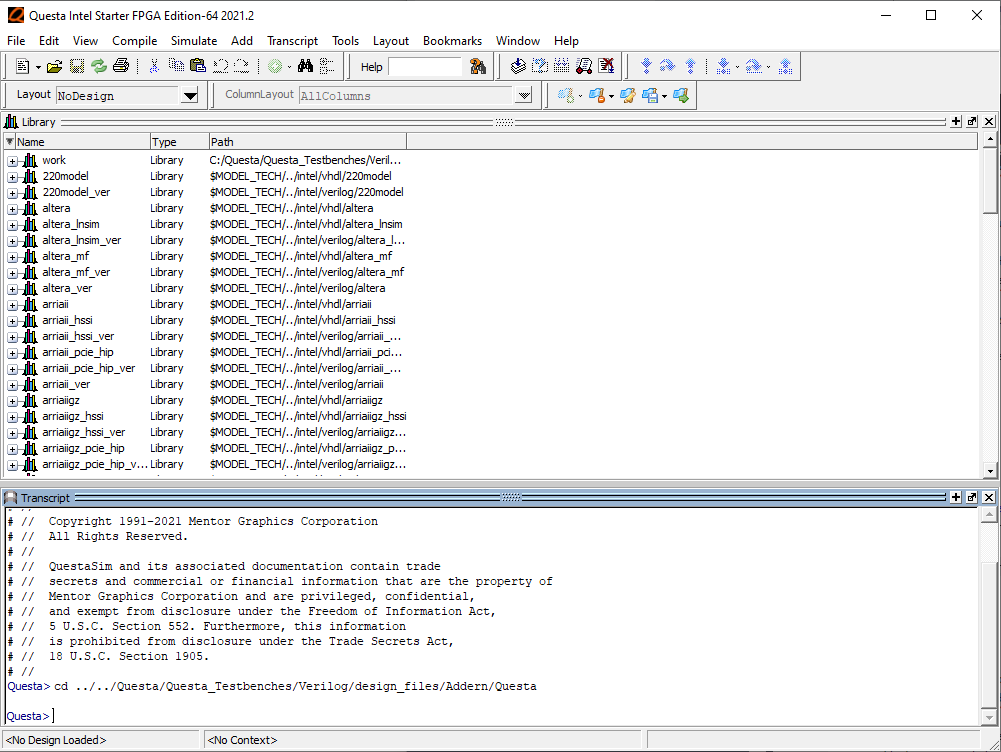
\includegraphics[width = .9\textwidth]{figures/gui1.png}
	\end{center}
		  \caption{The {\it Questa} window.}
	\label{fig:gui1}
\end{figure}

\noindent
Figure~\ref{fig:tcl} shows the contents of the script {\it testbench.tcl}. First, the
\texttt{quit} command is invoked to ensure that no simulation is already running. Then, in
Line~\ref{line:tcl2} the \texttt{vlib} command is executed to create a {\it work} design
library; Questa stores compilation/simulation results in this working library.   
The VHDL compiler is invoked in Line~\ref{line:tcl3} to
compile the source code for the {\it Addern} entity, which is in the {\it parent} folder (../),  
and in Line~\ref{line:tcl4} to compile {\it testbench.vht} in the current folder.
The simulation is started by the \texttt{vsim} command in Line~\ref{line:tcl5}. It includes some
simulation libraries for Intel FPGAs that may be needed by Questa.
If the included libraries aren't required for the current
design, then they will be ignored during the simulation. 
Line~\ref{line:tcl6} in Figure~\ref{fig:tcl} executes the command \texttt{do~wave.do}.
The {\it do} command is used to execute other Questa commands provided in a file. In
this case the file {\it wave.do}, which will be described shortly, contains various commands
that are used to configure the Questa waveform-display window. The final command in Figure~\ref{fig:do}
advances the simulation by a desired amount of time, which in this case is 120 ns.

\noindent
To run the script, in the {\it Transcript} window type the command
\texttt{do testbench.tcl}. Questa will execute the commands in this script and then
update its graphical user interface to show the simulation results. 
The updated Questa window after running the {\it testbench.tcl} script is illustrated 
in Figure~\ref{fig:gui2}.

\lstset{language=Tcl,numbers=left,escapechar=|}
\begin{figure}[h!]
\begin{center}
\begin{minipage}[t]{12.5 cm}
\begin{lstlisting}[name=tcl]
|\label{line:tcl0}|# stop any simulation that is currently running
|\label{line:tcl1}|quit -sim
# create the default "work" library
|\label{line:tcl2}|vlib work;

# compile the VHDL source code, and the testbench
|\label{line:tcl3}|vcom ../*.vhd
|\label{line:tcl4}|vcom *.vht
|\label{line:tcl5}|vsim work.testbench -Lf 220model -Lf altera_mf
|\label{line:tcl6}|do wave.do
|\label{line:tcl7}|run 120 ns
\end{lstlisting}
\end{minipage}
\caption{The {\it testbench.tcl} file.}
\label{fig:tcl}
\end{center}
\end{figure}
\begin{figure}[h!]
	\begin{center}
		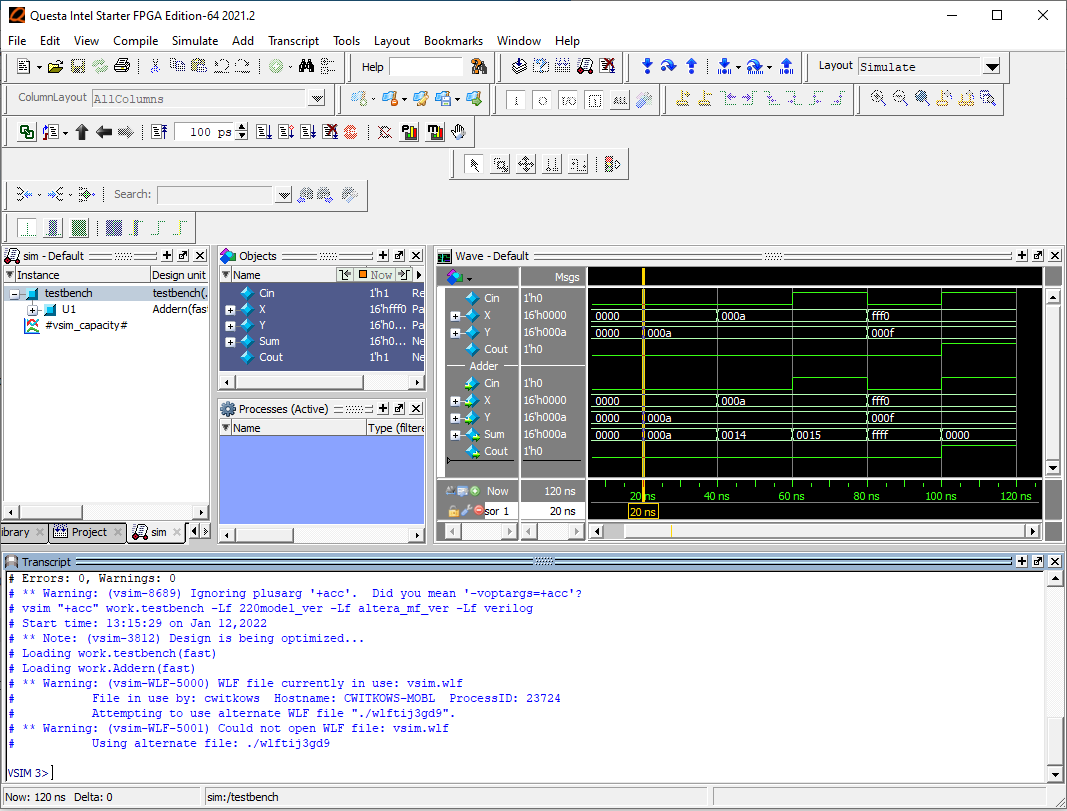
\includegraphics[width = .85\textwidth]{figures/gui2.png}
	\end{center}
		  \caption{The updated {\it Questa} window.}
	\label{fig:gui2}
\end{figure}

The {\it wave.do} file used for this design example appears in Figure~\ref{fig:do}. 
It specifies in Lines~\ref{line:do1} to \ref{line:do2}
which signal waveforms should be displayed in the simulation results, and 
also includes a number of settings related to the display. To add or delete waveforms 
in the display you can manually edit the {\it wave.do} file using any text editor, 
or you can select which waveforms should be displayed by using the Questa graphical 
user interface. Referring to Figure~\ref{fig:gui2}, changes to the displayed waveforms 
can be selected by right-clicking in the waveform window. Waveforms can be added to 
the display by selecting a signal in the \texttt{Objects} window and then 
{\it dragging-and-dropping} that signal name into the \texttt{Wave} window. 
A more detailed discussion about commands
available in the graphical user interface is provided in Appendix A.

\noindent
Quit the Questa software to complete this part of the tutorial. To quit the program you 
can either select the \texttt{File}~$>$~\texttt{Quit} command, or 
type \texttt{exit} in the {\it Transcript}
window, or just click on the \texttt{X} in the upper-right corner of the Questa window.

\lstset{numbers=left,escapechar=|}
\begin{figure}[h!]
\begin{center}
\begin{minipage}[h!]{14.5 cm}
\begin{lstlisting}[name=do]
onerror {resume}
quietly WaveActivateNextPane {} 0
|\label{line:do1}|add wave -noupdate -label Cin /testbench/Cin
add wave -noupdate -label X -radix hexadecimal /testbench/X
add wave -noupdate -label Y -radix hexadecimal /testbench/Y
add wave -noupdate -label Cout /testbench/Cout
add wave -noupdate -divider Adder
add wave -noupdate -label Cin /testbench/U1/Cin
add wave -noupdate -label X -radix hexadecimal /testbench/U1/X
add wave -noupdate -label Y -radix hexadecimal /testbench/U1/Y
add wave -noupdate -label Sum -radix hexadecimal /testbench/U1/Sum
|\label{line:do2}|add wave -noupdate -label Cout /testbench/U1/Cout
TreeUpdate [SetDefaultTree]
WaveRestoreCursors {{Cursor 1} {20000 ps} 0}
quietly wave cursor active 1
configure wave -namecolwidth 73
configure wave -valuecolwidth 64
configure wave -justifyvalue left
configure wave -signalnamewidth 0
configure wave -snapdistance 10
configure wave -datasetprefix 0
configure wave -rowmargin 4
configure wave -childrowmargin 2
configure wave -gridoffset 0
configure wave -gridperiod 1
configure wave -griddelta 40
configure wave -timeline 0
configure wave -timelineunits ns
update
WaveRestoreZoom {0 ps} {120 ns}
\end{lstlisting}
\end{minipage}
\caption{The {\it wave.do} file.}
\label{fig:do}
\end{center}
\end{figure}

\section{Simulating a Sequential Circuit}

Another Questa example, called {\it Accumulate}, is included as part of the
{\it design files} for this tutorial. Copy the {\it Accumulate} example to 
a folder on your computer, such as 
{\it C:$\backslash$Questa\_Tutorial$\backslash$Accumulate}. In the {\it Accumulate} folder
there is a VHDL source-code file called {\it Accumulate.vhd} and a subfolder named 
{\it Questa}. The {\it Accumulate.vhd} file, which provides the VHDL code that we will 
simulate, is shown in Figure~\ref{fig:accumulate}. It
represents the logic circuit illustrated in Figure~\ref{fig:circuit}, which includes an
adder, register, and down-counter. The purpose of this circuit is to add together, or
{\it accumulate}, values of the input {\it X} for each clock cycle until the counter 
reaches zero. 

\lstset{language=VHDL,numbers=none,escapechar=?}
\begin{figure}[hb!]
\begin{center}
\begin{minipage}[t]{15 cm}
\begin{lstlisting}[name=accumulate]
ENTITY Accumulate IS
   PORT ( KEY : IN STD_LOGIC_VECTOR(0 DOWNTO 0);
          SW : IN STD_LOGIC_VECTOR(9 DOWNTO 0);  
          CLOCK_50 : IN STD_LOGIC;
          LEDR : OUT STD_LOGIC_VECTOR(9 DOWNTO 0));
END ENTITY; 

ARCHITECTURE Behaviour OF Accumulate IS
   SIGNAL X, Y, Count : STD_LOGIC_VECTOR(4 DOWNTO 0); 
   SIGNAL Clock, Resetn, z : STD_LOGIC;
   SIGNAL Sum : STD_LOGIC_VECTOR(9 DOWNTO 0);
BEGIN
   Clock <= CLOCK_50;
   X <= SW(4 DOWNTO 0);
   Y <= SW(9 DOWNTO 5);
   Resetn <= KEY(0);
   PROCESS (Clock, Resetn, z)   -- define the Sum register
   BEGIN 
      IF Resetn = '0' THEN
         Sum <= "0000000000";
      ELSIF Clock'EVENT AND Clock = '1' AND z = '1' THEN
         Sum <= Sum + ("00000" & X);
      END IF;
   END PROCESS;

   PROCESS (Clock, Resetn, Y, z) -- define the down-counter
      BEGIN
         IF Resetn = '0' THEN
            Count <= Y;
         ELSIF Clock'EVENT AND Clock ='1' AND z = '1' THEN
            Count <= Count - "00001";
        END IF;
   END PROCESS;
   z <= Count(0) OR Count(1) OR Count(2) OR Count(3) OR Count(4);
   LEDR <= Sum(9 DOWNTO 0);
END Behaviour;
\end{lstlisting}
\end{minipage}
\caption{VHDL code for the accumulator.}
\label{fig:accumulate}
\end{center}
\end{figure}
\clearpage

\noindent
The {\it Accumulate} entity in Figure~\ref{fig:accumulate} has ports {\it KEY}, 
{\it CLOCK\_50}, {\it SW}, and {\it LEDR} because it is intended to be implemented
on a DE-series board that features an Intel FPGA, such as the {\it DE1-SoC} board. After 
simulating the VHDL code to verify its correct operation, you may
wish to compile it using the Quartus Prime CAD tools and then download and test the 
resulting circuit on a board.  

\noindent
A {\it testbench.vht} file for the accumulator design under test (DUT) is given in 
Figure~\ref{fig:tb2}. Three signals, {\it KEY}, {\it CLOCK\_50}, and 
{\it SW} are declared to provide inputs to the DUT, as well as a signal {\it LEDR}
for connecting to the DUT outputs. The {\it Accumulate} entity is instantiated in
Line~\ref{line:tb2_inst}.
It is useful to define a periodic signal that can be used as a clock input for 
the {\it Accumulate} sequential circuit. We could manually define some number of cycles 
for such a signal in a process, but this method would be
awkward. Instead, Lines~\ref{line:tb2_clk0} to~\ref{line:tb2_clk1} in 
Figure~\ref{fig:tb2} show how to make a periodic signal by specifying just one period. 
This process gets executed repeatedly, because it does not end with a sepatate 
\texttt{WAIT} statement.  Thus, the {\it CLOCK\_50} signal is inverted
every 10~ns in simulation time to create a 50 MHz periodic waveform. This clock 
process is executed {\it concurrently} by the Simulator along with the process in
Lines~\ref{line:tb2_v1} to~\ref{line:tb2_v2}. This process sets 
{\it KEY}$_0 = 0$ and {\it SW}$=0$
at the start of the simulation, which allows the {\it Sum} in the accumulator to be
cleared. At 20~ns in simulation time {\it SW}$_{9-5}$ is set to 10, so that this value can 
be loaded into the counter. Finally, at 40~ns in simulation time {\it KEY}$_0$
is set to 1 and {\it SW}$_{4-0}$ is set to 30, so that this value can be
{\it accumulated} for each clock cycle until the counter reaches~0.

\begin{figure}[h!]
	\begin{center}
		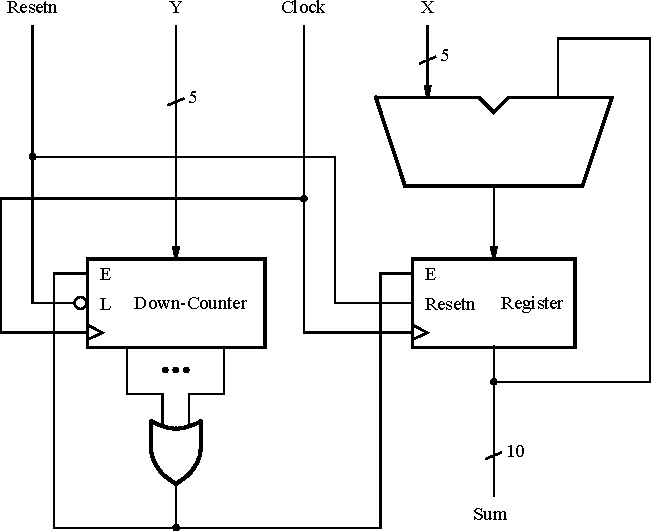
\includegraphics[scale = 1.0]{figures/figaccum.pdf}
	\end{center}
		  \caption{The accumulator circuit.}
	\label{fig:circuit}
\end{figure}

\noindent
Reopen the {\it Questa} software to get to the window in Figure~\ref{fig:gui1}.
Click on the {\it Transcript} window at the bottom of the figure and then use the
\texttt{cd} command to navigate to the Questa folder for the accumulator. For 
example, in our case we would type 
\texttt{cd C:/Questa\_Tutorial/Accumulate/Questa}. 
Then, in the {\it Transcript} window type the command \texttt{do testbench.tcl} as you
did for the previous example. The {\it testbench.tcl} script for this example is identical
to the one shown in Figure~\ref{fig:tcl}, except that the last line specifies
\texttt{run 300 ns}.

\lstset{language=VHDL,numbers=left,escapechar=|}
\begin{figure}[h!]
\begin{center}
\begin{minipage}[t]{15 cm}
\begin{lstlisting}[name=testbench2]
ENTITY testbench IS
END testbench;
 
ARCHITECTURE Behavior OF testbench IS
    COMPONENT Accumulate
       PORT ( KEY : IN STD_LOGIC_VECTOR(0 DOWNTO 0);
              SW : IN STD_LOGIC_VECTOR(9 DOWNTO 0);  
              CLOCK_50 : IN STD_LOGIC;
              LEDR : OUT STD_LOGIC_VECTOR(9 DOWNTO 0));
    END COMPONENT;

    SIGNAL CLOCK_50 : STD_LOGIC;
    SIGNAL KEY : STD_LOGIC_VECTOR(0 DOWNTO 0);
    SIGNAL SW : STD_LOGIC_VECTOR(9 DOWNTO 0);
    SIGNAL LEDR : STD_LOGIC_VECTOR(9 DOWNTO 0);
BEGIN
|\label{line:tb2_inst}|U1: Accumulate PORT MAP (KEY, SW, CLOCK_50, LEDR);

|\label{line:tb2_clk0}|    clock_process: PROCESS
    BEGIN
        CLOCK_50 <= '0';
        WAIT FOR 10 ns;
        CLOCK_50 <= '1';
        WAIT FOR 10 ns;
|\label{line:tb2_clk1}|    END PROCESS;

|\label{line:tb2_v1}|    vectors: PROCESS
    BEGIN
        KEY(0) <= '0'; SW <= "0000000000"; 
        WAIT FOR 20 ns;
        SW(9 DOWNTO 5) <= "01010";
        WAIT FOR 20 ns;
        SW(4 DOWNTO 0) <= "11110"; 
        KEY(0) <= '1';
        WAIT;
|\label{line:tb2_v2}|    END PROCESS;
END;
\end{lstlisting}
\end{minipage}
\caption{The VHDL testbench code for the sequential circuit.}
\label{fig:tb2}
\end{center}
\end{figure}

\noindent
The simulation results for our sequential circuit, which display the waveforms selected in its
{\it wave.do} file, appear in Figure~\ref{fig:gui3}. In this figure the {\it SW} and 
{\it LEDR} signals are displayed in hexadecimal, while {\it X}, {\it Sum}, {\it Y}, and {\it
Count} are displayed as unsigned (decimal) values. The {\it Sum} is cleared by the 
clock edge at 10~ns, and the {\it Count} is initialized to 10 at 30~ns. Starting with the clock
edge at 50~ns the value $X=30$ is accumulated until the counter reaches 0.

\noindent
Quit the Questa software to complete this part of the tutorial.

\begin{figure}[h!]
	\begin{center}
		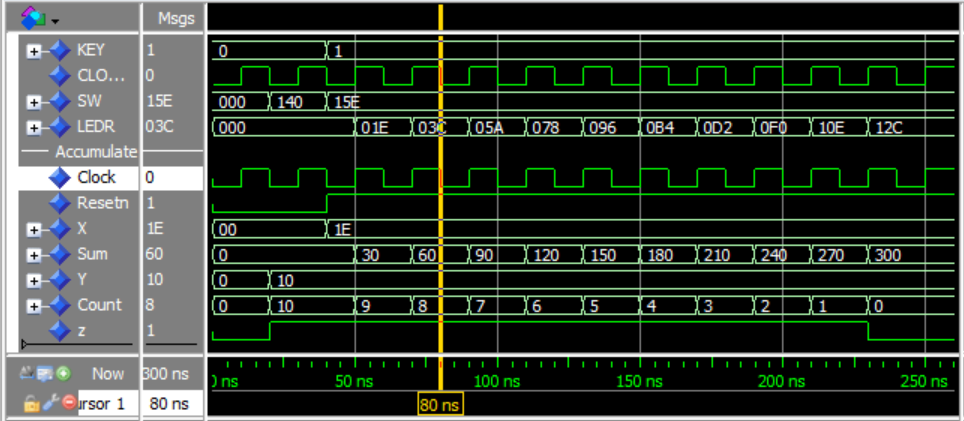
\includegraphics[width = \textwidth]{figures/gui3.png}
	\end{center}
		  \caption{The simulation results for our sequential circuit.}
	\label{fig:gui3}
\end{figure}

\section{Simulating a Circuit that Includes a Memory Module}

The {\it design files} archive provided along with this tutorial includes a Questa example 
called {\it Display}. It shows how to instantiate a memory module in VHDL code, and how
to initialize the stored contents of the memory in a Questa simulation. Copy the {\it Display}
files to a folder on your computer, such as 
{\it C:$\backslash$Questa\_Tutorial$\backslash$Display}. 
In the {\it Display} folder there is a file called {\it Display.vhd}
that provides the VHDL code that we will simulate, and 
a subfolder named {\it Questa}.

\noindent
Figure~\ref{fig:display} shows the VHDL code for {\it Display.vhd}.
Its ports are named {\it KEY}, {\it SW}, {\it HEX0}, and {\it LEDR} because the entity is intended 
to be implemented on a DE-series board that features an Intel FPGA, such as the {\it DE1-SoC}
board. After simulating the VHDL code to verify its correct operation, you may
wish to compile it using the Quartus Prime CAD tools and then download and test the 
resulting circuit on a board.  

\noindent
Figure~\ref{fig:memory}$a$ gives a logic circuit that corresponds to the code in 
Figure~\ref{fig:display}. The circuit contains a counter that is used to read the 
contents of successive addresses from a memory. This memory provides codes in ASCII format 
for some upper- and lower-case letters, which are provided as inputs to a decoder entity. 
The counter and memory module have a common clock signal, and the counter has a
synchronous clear input. Each successive clock cycle advances the counter and reads 
a new ASCII code from the memory. Since the counter is three-bits wide, only the first 
eight locations in the memory are read (the upper two address bits on the memory are set
to 00), and they provide the ASCII codes for letters A, b, C, d, E, F, g, and h. The 
decoder produces an appropriate bit-pattern to render each letter on a seven-segment display.
The memory used in the logic circuit is depicted in part $b$ of Figure~\ref{fig:memory}. It
is a $32 \times 8$ synchronous read-only memory (ROM), which has a register for holding 
address values. The memory is initialized with the contents of the file {\it inst\_mem.mif},
which is illustrated in Figure~\ref{fig:mif}. This file contains the ASCII codes for the 
eight letters displayed by the circuit.

\lstset{language=VHDL,numbers=none,escapechar=?}
\begin{figure}[h!]
\begin{center}
\begin{minipage}[t]{15 cm}
\begin{lstlisting}[name=display]
ENTITY display IS
    PORT ( KEY : IN STD_LOGIC_VECTOR(0 DOWNTO 0);
           SW : IN STD_LOGIC_VECTOR(0 DOWNTO 0);  
           HEX0 : OUT STD_LOGIC_VECTOR(6 DOWNTO 0);
           LEDR : OUT STD_LOGIC_VECTOR(9 DOWNTO 0) );
END ENTITY; 

ARCHITECTURE Behavior OF display IS
    COMPONENT inst_mem 
        PORT ( address   : IN STD_LOGIC_VECTOR (4 DOWNTO 0);
               clock     : IN STD_LOGIC ;
               q         : OUT STD_LOGIC_VECTOR (7 DOWNTO 0));
    END COMPONENT;
    COMPONENT count3
        PORT ( Resetn, Clock   : IN   STD_LOGIC;
               Q               : OUT  STD_LOGIC_VECTOR(2 DOWNTO 0));
    END COMPONENT;

    CONSTANT A : STD_LOGIC_VECTOR(7 DOWNTO 0) := x"41";
    CONSTANT b : STD_LOGIC_VECTOR(7 DOWNTO 0) := x"62";
    CONSTANT C : STD_LOGIC_VECTOR(7 DOWNTO 0) := x"43";
    CONSTANT d : STD_LOGIC_VECTOR(7 DOWNTO 0) := x"64";
    CONSTANT E : STD_LOGIC_VECTOR(7 DOWNTO 0) := x"45";
    CONSTANT F : STD_LOGIC_VECTOR(7 DOWNTO 0) := x"46";
    CONSTANT g : STD_LOGIC_VECTOR(7 DOWNTO 0) := x"67";
    CONSTANT h : STD_LOGIC_VECTOR(7 DOWNTO 0) := x"68";
    SIGNAL Resetn, Clock : STD_LOGIC;
    SIGNAL Count : STD_LOGIC_VECTOR(2 DOWNTO 0);
    SIGNAL Address : STD_LOGIC_VECTOR(4 DOWNTO 0);
    SIGNAL char : STD_LOGIC_VECTOR(7 DOWNTO 0);
BEGIN 
    Resetn <= SW(0);
    Clock <= KEY(0);

    U1: count3 PORT MAP (Resetn, Clock, Count);
    Address <= "00" & Count;
    U2: inst_mem PORT MAP (Address, Clock, char);
    LEDR <= "00" & char;
    
    HEX0 <= "0001000" WHEN char = A ELSE
            "0000011" WHEN char = b ELSE
            "1000110" WHEN char = C ELSE
            "0100001" WHEN char = d ELSE
            "0000110" WHEN char = E ELSE
            "0001110" WHEN char = F ELSE
            "0010000" WHEN char = g ELSE
            "0001011" WHEN char = h ELSE
            "1111111";
END Behavior;
\end{lstlisting}
\end{minipage}
\caption{VHDL code for the display circuit.}
\label{fig:display}
\end{center}
\end{figure}
\clearpage
\newpage

\begin{figure}[t]
	\begin{center}
		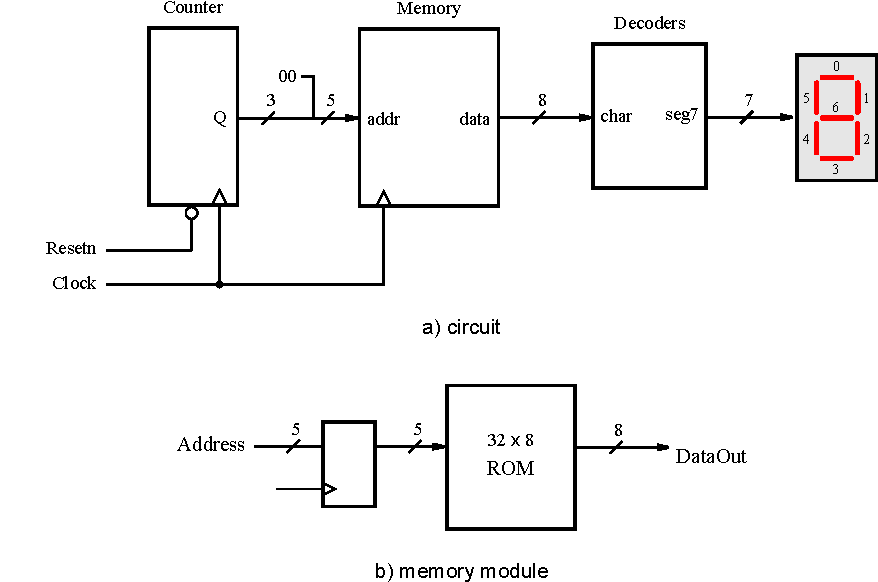
\includegraphics[scale = 1.0]{figures/figdisplay.pdf}
	\end{center}
		  \caption{The circuit for the memory example.}
	\label{fig:memory}
\end{figure}

\begin{figure}[bh!]
\begin{center}
\begin{minipage}[t]{12.5 cm}
\begin{tabbing}
DEPTH = 32;\\
WIDTH = 8;\\
ADDRESS\_RADIX = HEX;\\
DATA\_RADIX = DEC;\\
CONTENT\\
BEGIN\\
BEGI\=00X\=: \=104;XXXX\=\% A \=\% \kill
\>00 \>: \>65;    \>\% A \>\%\\
\>01 \>: \>98;    \>\% b \>\%\\
\>02 \>: \>67;    \>\% C \>\%\\
\>03 \>: \>100;   \>\% d \>\%\\
\>04 \>: \>69;    \>\% E \>\%\\
\>05 \>: \>70;    \>\% F \>\%\\
\>06 \>: \>103;   \>\% g \>\%\\
\>07 \>: \>104;   \>\% h \>\%\\
END;
\end{tabbing}
\end{minipage}
\end{center}
    \caption{The {\it inst\_mem.mif} memory initialization file.}
\label{fig:mif}
\end{figure}

\newpage
\noindent
A {\it testbench.vht} file for the {\it Display} design under test (DUT) is given in 
Figure~\ref{fig:tb3}. Two signals, {\it KEY} and {\it SW} are declared to provide 
inputs to the DUT, as well as two signals {\it HEX0} and {\it LEDR}
for connecting to the DUT outputs. The DUT is instantiated in Line~\ref{line:disp} of 
the testbench. It 
uses a process to create a clock waveform with a 20~ns period on the {\it KEY} signal.  Another 
process is used to perform a synchronous reset of the counter with the SW signal. 

\lstset{language=VHDL,numbers=left,escapechar=|}
\begin{figure}[h]
\begin{center}
\begin{minipage}[t]{12.5 cm}
\begin{lstlisting}[name=testbench3]
ENTITY testbench IS
END testbench;
 
ARCHITECTURE Behavior OF testbench IS
    COMPONENT display
        PORT ( KEY   : IN   STD_LOGIC_VECTOR(0 DOWNTO 0);
               SW    : IN   STD_LOGIC_VECTOR(0 DOWNTO 0);
               HEX0  : OUT  STD_LOGIC_VECTOR(6 DOWNTO 0);
               LEDR  : OUT  STD_LOGIC_VECTOR(9 DOWNTO 0));
    END COMPONENT;

    SIGNAL KEY : STD_LOGIC_VECTOR(0 DOWNTO 0);
    SIGNAL SW : STD_LOGIC_VECTOR(0 DOWNTO 0);
    SIGNAL HEX0 : STD_LOGIC_VECTOR(6 DOWNTO 0);
    SIGNAL LEDR : STD_LOGIC_VECTOR(9 DOWNTO 0);
BEGIN
    |\label{line:disp}|U1: display PORT MAP (KEY, SW, HEX0, LEDR);

    clock_process: PROCESS
    BEGIN
        KEY(0) <= '0';
        WAIT FOR 10 ns;
        KEY(0) <= '1';
        WAIT FOR 10 ns;
    END PROCESS;    
    
    vectors: PROCESS
    BEGIN
        SW(0) <= '0';       -- Resetn = 0
        WAIT FOR 20 ns;     
        SW(0) <= '1';       -- Resetn = 1
        WAIT;
    END PROCESS;
END;
\end{lstlisting}
\end{minipage}
\caption{Testbench code for the memory example.}
\label{fig:tb3}
\end{center}
\end{figure}

\noindent
Figure~\ref{fig:tcl2} shows the contents of the script {\it testbench.tcl} for this example.
It has the same structure as the file shown in Figure~\ref{fig:tcl}, with two exceptions. 
First, in Lines~\ref{line:tcl2_1} to~\ref{line:tcl2_2} the script checks whether there 
exists an {\it inst\_mem.mif} memory initialization file in the parent folder; if so, 
it copies this file to the Questa folder so that the memory will be properly initialized
during simulation. Second, in Lines~\ref{line:tcl2_3} 
to~\ref{line:tcl2_4} the script checks if an ``empty black box'' file, which can 
optionally be created by the Quartus software, exists in the parent directory. 
If so, the script deletes this file, because it would cause an error during simulation.

\lstset{language=Tcl,numbers=left,escapechar=|}
\begin{figure}[h!]
\begin{center}
\begin{minipage}[h]{15 cm}
\begin{lstlisting}[name=tcl2]
quit -sim

# if simulating with a MIF file, copy it. Assumes inst_mem.mif
|\label{line:tcl2_1}|if {[file exists ../inst_mem.mif]} {
	file delete inst_mem.mif
	file copy ../inst_mem.mif .
|\label{line:tcl2_2}|}
# if Quartus generated an "empty black box" file, delete it
|\label{line:tcl2_3}|if {[file exists ../inst_mem_bb.vhd]} {
	file delete ../inst_mem_bb.vhd
|\label{line:tcl2_4}|}
# create the default "work" library
vlib work;

# compile the VHDL source code in the parent folder
vcom ../*.vhd
# compile the VHDL code of the testbench
vcom *.vht
# start the Simulator, including some libraries
vsim work.testbench -Lf 220model -Lf altera_mf
# show waveforms specified in wave.do
do wave.do
run 180 ns
\end{lstlisting}
\end{minipage}
\caption{The {\it testbench.tcl} file.}
\label{fig:tcl2}
\end{center}
\end{figure}

\noindent
Reopen the {\it Questa} software to get to the window in Figure~\ref{fig:gui1}.
In the {\it Transcript} window use the \texttt{cd} command to navigate to the 
Questa folder for the this part of the tutorial. For example, in our 
case we would type \texttt{cd C:/Questa\_Tutorial/Display/Questa}. 
In the {\it Transcript} window type the command \texttt{do~testbench.tcl} to run
the script in Figure~\ref{fig:tcl2}.
The simulation results for our circuit, which display the waveforms selected in its
{\it wave.do} file, appear in Figure~\ref{fig:gui4}.It shows in the {\it char} 
waveform, displayed using the ``radix'' ASCII, the values read from each address in memory.
These values are also shown in hexadecimal in the {\it LEDR} waveform, and the 
decoder outputs are shown in binary in the {\it HEX0} waveform.

\begin{figure}[h!]
	\begin{center}
		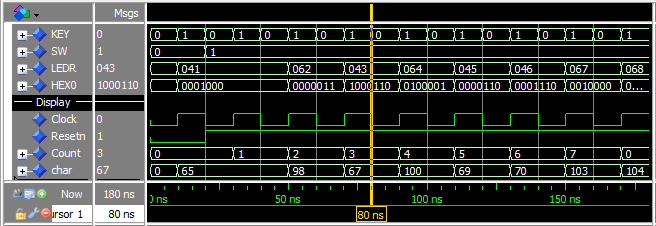
\includegraphics[width = 0.95\textwidth]{figures/display.png}
	\end{center}
		  \caption{The simulation results for our memory example.}
	\label{fig:gui4}
\end{figure}

\section{Setting up a Questa Simulation}

The files described above can be used as a starting point for setting up your own Questa 
simulation, as follows.  In the folder that contains your VHDL source-code to be
simulated, make a subfolder named {\it Questa}. 
Copy into this subfolder the files {\it testbench.vht},
{\it testbench.tcl}, and {\it wave.do} from one of the examples above. Then, 
modify {\it testbench.vht} to instantiate your top-level VHDL entity and create whatever 
waveforms are needed. You can use an identical {\it testbench.tcl} script as shown above, 
except that you might want to specify a different amount of simulation time for 
the \texttt{run} command. Since the .{\it vht} and .{\it tcl} files are ASCII text
files, you can edit them with any text editor of your choosing (or the text editor
provided within Questa). Finally, 
modify the {\it wave.do} file to choose the waveforms that should be displayed.
You can change the {\it wave.do} file manually by editing it with a text editor, or you can 
make use of the commands available in the Questa graphical user interface, 
as discussed in Appendix A.

\newpage
\section*{Appendix A: Using the Questa Graphical User Interface}

This appendix illustrates some of the features available in the Questa graphical user
interface for displaying waveforms. We will show how to add waveforms to the Questa
window, and how to change the properties of a waveform, such as its displayed name 
and number radix.

As an example we will show how waveforms can be added to the Questa display for the
{\it accumulator} circuit from the previous section. Figure \ref{fig:appa_fig1} displays the 
Questa window for this circuit before any waveforms have been selected.

\begin{figure}[h!]
	\begin{center}
		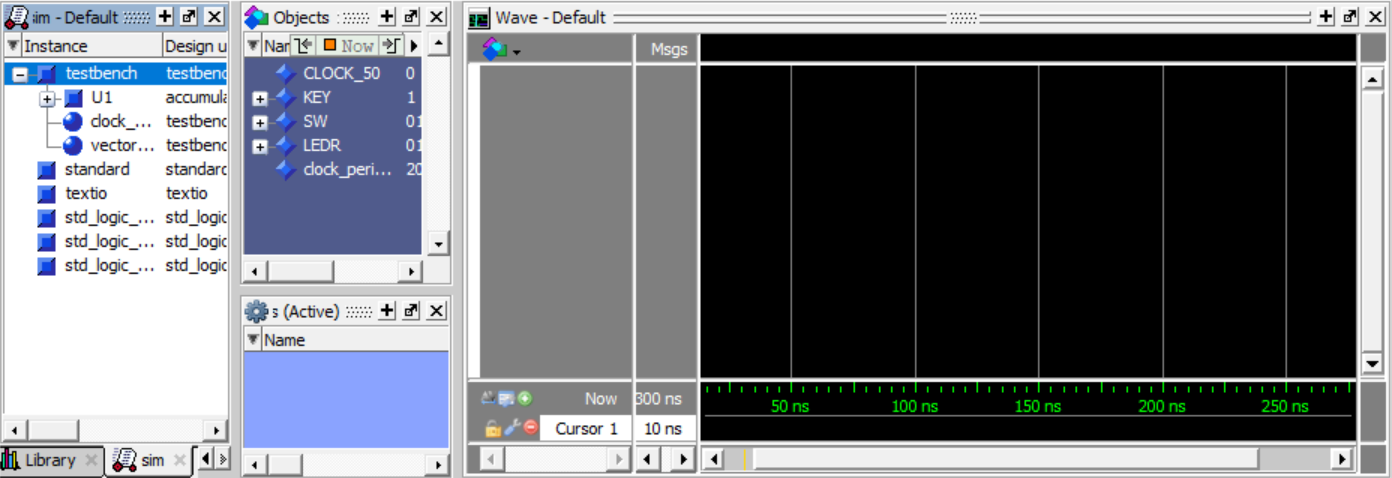
\includegraphics[width = \textwidth]{figures/appa_fig1.png}
	\end{center}
		  \caption{The {\it Questa} waveform display.}
	\label{fig:appa_fig1}
\end{figure}

\noindent
In Figure \ref{fig:appa_fig2} we have selected a waveform, as follows. First, we clicked
on the \texttt{testbench} entity in the upper left part of the display. As a result of
this action the signals that exist in the selected entity are listed in the \texttt{Objects}
pane (the area with the dark blue background). In this list we then used the 
left mouse button to {\it drag-and-drop} the \texttt{KEY} signal name from the 
\texttt{Objects} list into the \texttt{Wave} window. Then, as illustrated in the figure, we 
right-clicked on the name of the signal in the \texttt{Wave} display, which is 
\texttt{/testbench/KEY}, and then clicked on \texttt{Properties} to open the window in 
Figure \ref{fig:appa_fig3}.

\begin{figure}[h!]
	\begin{center}
		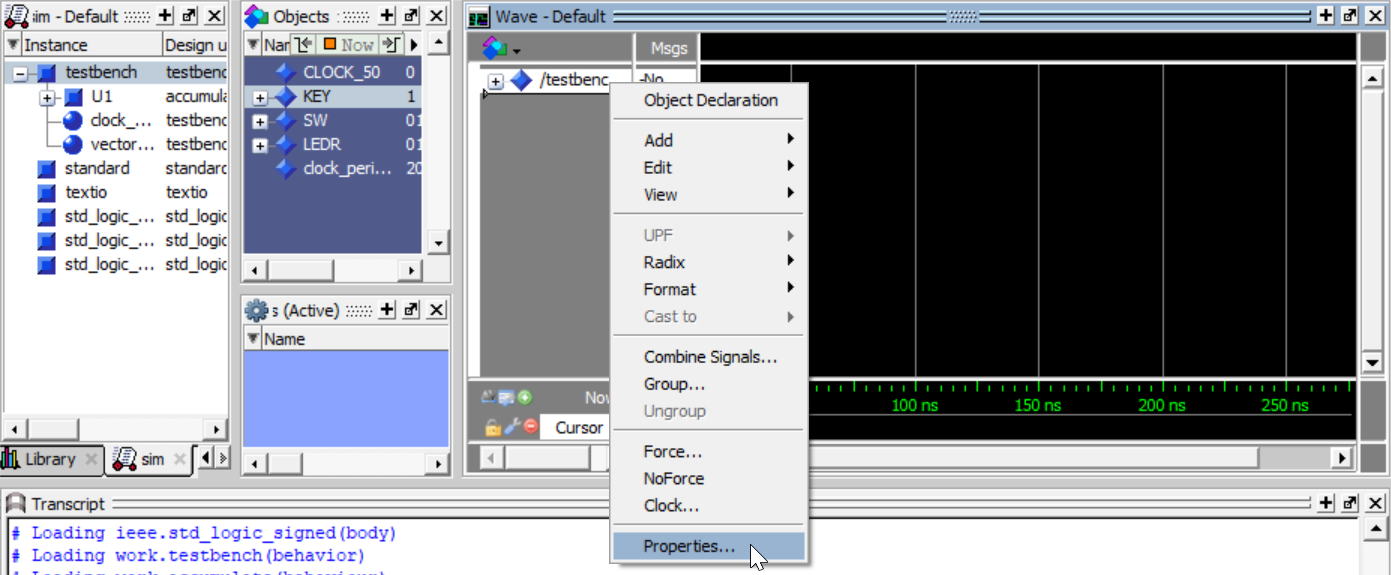
\includegraphics[width = \textwidth]{figures/appa_fig2.png}
	\end{center}
		  \caption{Adding a waveform from the testbench entity.}
	\label{fig:appa_fig2}
\end{figure}

\begin{figure}[h]
	\begin{center}
		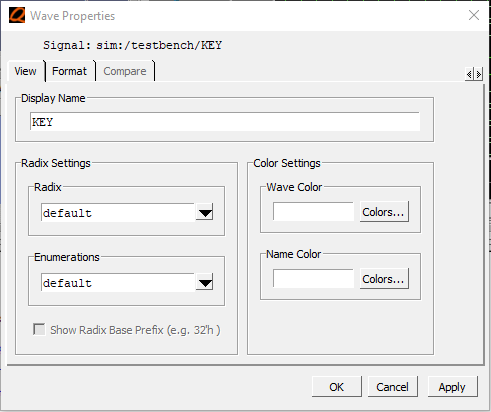
\includegraphics[scale=0.8]{figures/appa_fig3.png}
	\end{center}
		  \caption{Specifying a display name for a waveform.}
	\label{fig:appa_fig3}
\end{figure}

\noindent
In Figure \ref{fig:appa_fig3} we assigned the name \texttt{KEY} to the waveform, clicked
\texttt{Apply} and then closed this dialogue. We then used the same drag-and-drop mechanism
to add the signals \texttt{CLOCK\_50}, \texttt{SW}, and \texttt{LEDR} from the
\texttt{testbench} entity to the \texttt{Wave} window, and set convenient display names 
for these waveforms. The updated \texttt{Wave} window is shown in Figure \ref{fig:appa_fig4}.

\begin{figure}[h!]
	\begin{center}
		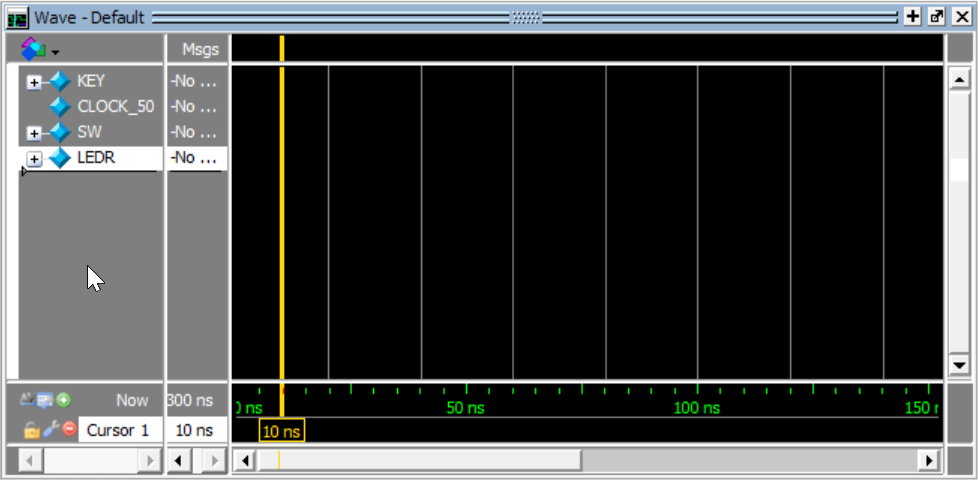
\includegraphics[width = \textwidth]{figures/appa_fig4.png}
	\end{center}
	\caption{The waveform display after adding more {\it testbench} signals.}
	\label{fig:appa_fig4}
\end{figure}

\noindent
Next, we wish to add signals from the \texttt{Accumulate} entity to the \texttt{Wave} window. 
But first we can add a {\it divider}, as a visual aid that separates the \texttt{testbench} 
signals and the \texttt{Accumulate} entity signals. A divider can be added by
right-clicking on the \texttt{Wave} window, as indicated in the Figure \ref{fig:appa_fig5}, 
clicking on \texttt{Add} in the pop-up menu, and then selecting \texttt{New Divider} to 
open the window in Figure~\ref{fig:appa_fig6}. 

\begin{figure}[h!]
	\begin{center}
		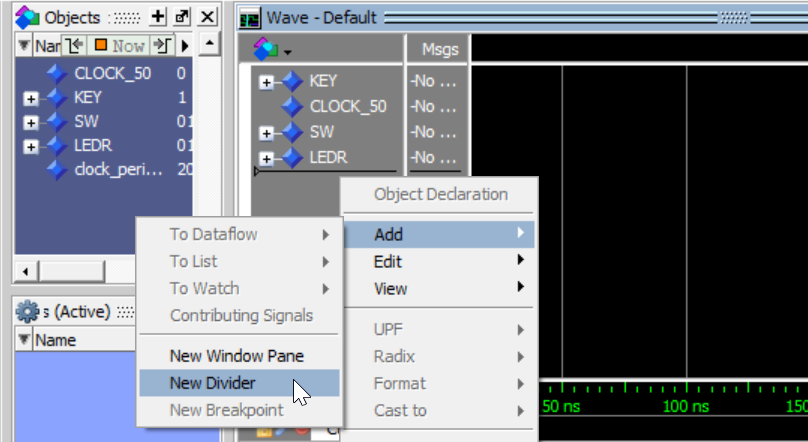
\includegraphics[]{figures/appa_fig5.png}
	\end{center}
		  \caption{Adding a divider to the waveform display.}
	\label{fig:appa_fig5}
\end{figure}

\noindent
We assigned \texttt{Accumulate} as the divider name in Figure~\ref{fig:appa_fig6},
and then closed this dialogue. The \texttt{Wave} window now appears as shown in 
Figure~\ref{fig:appa_fig7}.

\begin{figure}[h!]
	\begin{center}
		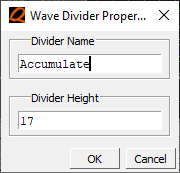
\includegraphics[scale=0.8]{figures/appa_fig6.png}
	\end{center}
		  \caption{Assigning a name to the divider.}
	\label{fig:appa_fig6}
\end{figure}

\begin{figure}[h!]
	\begin{center}
		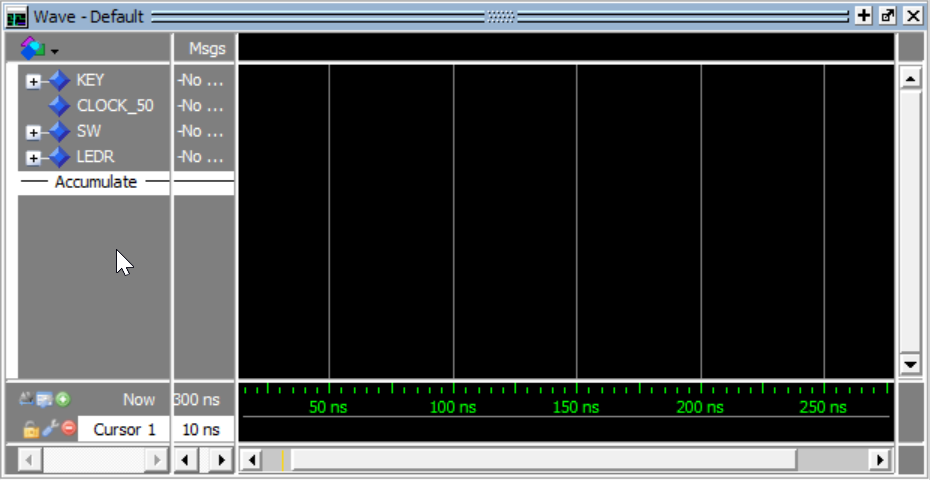
\includegraphics[width = \textwidth]{figures/appa_fig7.png}
	\end{center}
	\caption{The waveform display after adding the \texttt{Accumulate} divider.}
	\vspace{-0.25 cm}
	\label{fig:appa_fig7}
\end{figure}

\noindent
To add signals from the \texttt{Accumulate} entity to the \texttt{Wave} window we need to
click on the \texttt{U1} instance name of the \texttt{Accumulate} model, as indicated  
on the left-hand side of Figure~\ref{fig:appa_fig8}. The signals available in this entity
are then listed in the \texttt{Objects} pane. To obtain the display in the figure, we
used the drag-and-drop mechanism, and the \texttt{Wave Properties} dialogue, described 
previously, to add the \texttt{Clock}, \texttt{Resetn}, \texttt{X}, \texttt{Sum},
\texttt{Y}, \texttt{Count}, and \texttt{z} signals to the \texttt{Wave} window.

We now wish to perform a simulation of our \texttt{testbench} so that waveforms will be 
generated and shown for our selected signals. 
However, it is {\it critical} to first {\it save} the selections
that have been made in the \texttt{Wave} display to the {\it wave.do} file. If you run a 
simulation {\it without} first performing a save to the {\it wave.do} file, then all 
changes made to the \texttt{Wave} window will be discarded and lost!  

\begin{figure}[h!]
	\begin{center}
		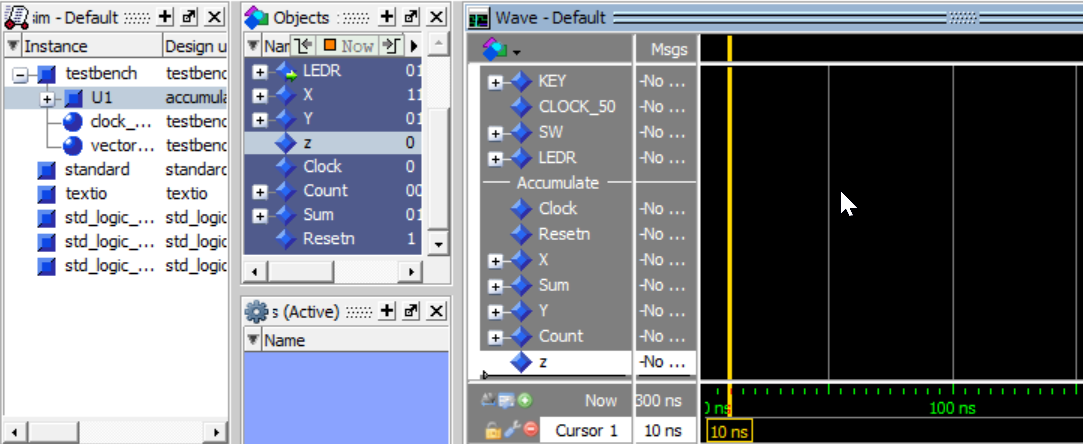
\includegraphics[width = \textwidth]{figures/appa_fig8.png}
	\end{center}
		  \caption{The waveform display after adding signals from the accumulate entity.}
	\label{fig:appa_fig8}
\end{figure}

\noindent
The command \texttt{File > Save Format} opens the dialogue shown in Figure~\ref{fig:appa_fig9}.
After clicking \texttt{OK} and then overwriting the {\it wave.do} file, the testbench 
simulation can be executed by typing the command \texttt{do testbench.tcl}. The resulting
waveform display is illustrated in Figure~\ref{fig:appa_fig10}. In this figure we
right-clicked on the \texttt{Wave} window and selected \texttt{Zoom Range} to open the
dialogue in Figure~\ref{fig:appa_fig11}. As indicated in the figure, we select a time range 
from 0 to 300 ns for the Wave display.

\begin{figure}[h!]
	\begin{center}
		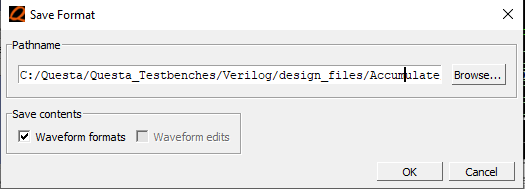
\includegraphics[scale=0.8]{figures/appa_fig9.png}
	\end{center}
	\caption{The \texttt{Save Format} dialogue.}
	\label{fig:appa_fig9}
\end{figure}

\begin{figure}[h!]
	\begin{center}
		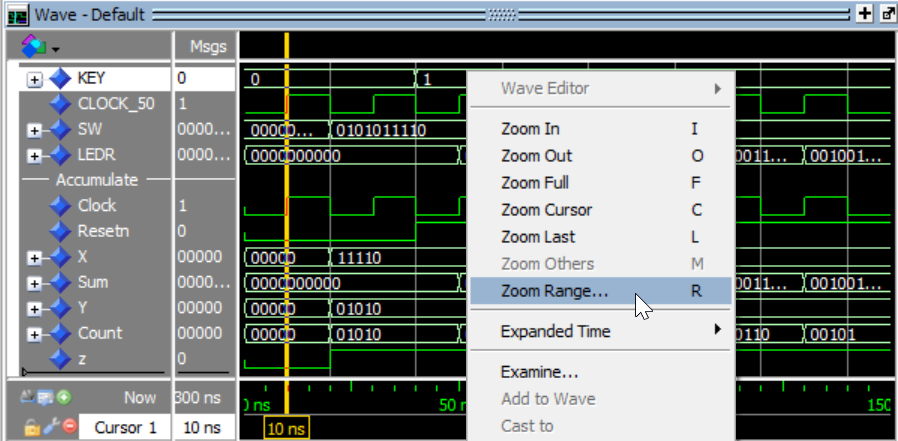
\includegraphics[scale=0.8]{figures/appa_fig10.png}
	\end{center}
		  \caption{The display after running the simulation; changing the zoom range.}
	\label{fig:appa_fig10}
\end{figure}

\begin{figure}[h!]
	\begin{center}
		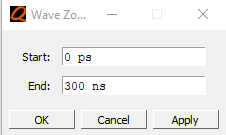
\includegraphics[scale=0.8]{figures/appa_fig11.png}
	\end{center}
		  \caption{Inputting the zoom range.}
	\label{fig:appa_fig11}
\end{figure}

\noindent
To make it easier to see the values of signals in the \texttt{Wave} window, you can select
radices other than binary, which is the default. For example, in
Figure~\ref{fig:appa_fig12} we right-clicked on the \texttt{SW} signal, clicked on
\texttt{Radix}, and then selected \texttt{Hexadecimal}. After setting the radix to
hexadecimal for several additional signals, the final \texttt{Wave} display appears as
illustrated in Figure~\ref{fig:appa_fig13}.
As mentioned earlier, changes to the waveforms
have to be saved by using the \texttt{File > Save Format} command.

\begin{figure}[h!]
	\begin{center}
		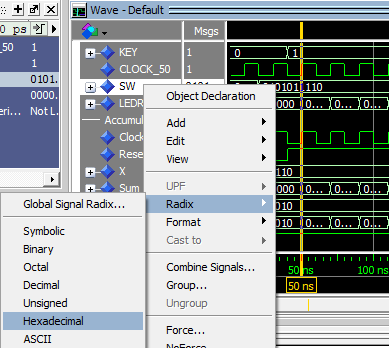
\includegraphics[scale=1.25]{figures/appa_fig12.png}
	\end{center}
		  \caption{Setting the radix for a waveform.}
	\label{fig:appa_fig12}
\end{figure}

\begin{figure}[h!]
	\begin{center}
		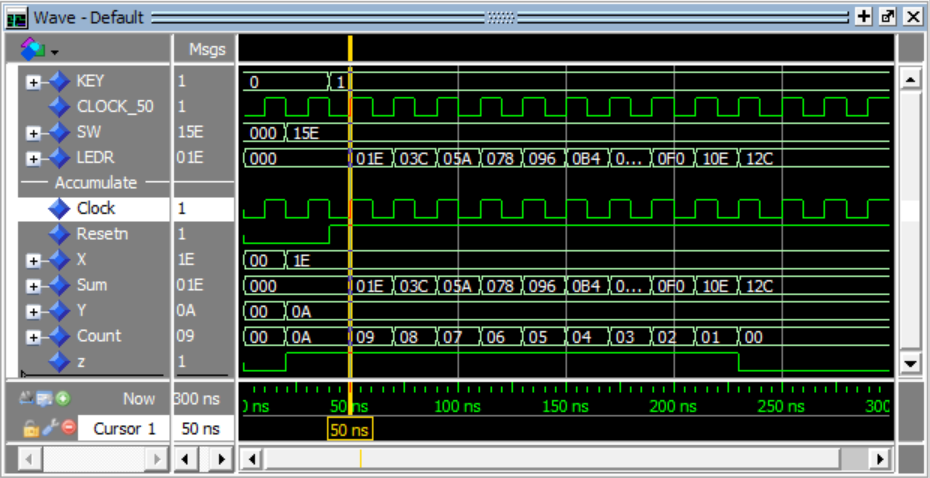
\includegraphics[scale=0.8]{figures/appa_fig13.png}
	\end{center}
		  \caption{The final waveform display.}
	\label{fig:appa_fig13}
\end{figure}

\noindent
This tutorial has described only a subset of the commands that are provided in the
Questa graphical user interface. Although a discussion of other available commands is 
beyond the scope of this tutorial, a number of more detailed Questa tutorials can be 
found by searching for them on the Internet.

% Copyright

%\newcommand{\datePublished}{Mar 2022}

\newcommand{\versnum}{21.1} %version number quartus/AMP
\newcommand{\quartusname}{Quartus\textsuperscript{\textregistered} Prime}	
\newcommand{\textBar}{For \quartusname{} \versnum{}}
\newcommand{\thisyear}{2022 } %for copyright
\newcommand{\company}{FPGAcademy.org}
\newcommand{\longteamname}{FPGAcademy.org}
\newcommand{\teamname}{FPGAcademy}
\newcommand{\website}{FPGAcademy.org}

\newcommand{\productAcronym}{AMP}
\newcommand{\productNameShort}{Monitor Program}

\newcommand{\productNameMedTM}{Monitor Program}
\newcommand{\productNameMed}{Monitor Program}

%\newcommand{\headerLogoFilePath}[1]{#1/FPGAcademy.png}



%%%%%%%%%%%%%%%%%%%%%%%%%%%%%%%%%%%%%%%%
%%% FPGAcademy Copyright Information %%%
%%%%%%%%%%%%%%%%%%%%%%%%%%%%%%%%%%%%%%%%

%Always put the copyright on a new page (clear page), with some vertical space from top
\clearpage
\vspace{1in}

\noindent

Copyright {\copyright} FPGAcademy.org. All rights reserved. FPGAcademy and the FPGAcademy logo are trademarks of  FPGAcademy.org.  This document is being provided on an ``as-is'' basis and as an accommodation and therefore all warranties, representations or guarantees of any kind (whether express, implied or statutory) including, without limitation, warranties of merchantability, non-infringement, or fitness for a particular purpose, are specifically disclaimed.

%FPGAcademy assumes no responsibility or liability arising out of the application or use of any information,  product,  or  service  described  herein  except  as  expressly  agreed  to  in  writing  by  FPGAcademy.



**Other names and brands may be claimed as the property of others.




\end{document}
